
As noted in the previous section, the k-d tree build process is by far the most expensive operation, and we would save a lot of time by managing to parallelize it.

One could think, why not use the same algorithm as in the serial case. This is a intuitive choice, but since the environment has changed the optimal algorithm may have changed as well. This is specialty true for our implementation, Algorithm~\ref{alg:seriel_tree_build}, since in a CUDA context a recursive algorithm is hard to parallelize. CUDA is based on a massive number of lightweight threads, and to get a fast algorithm one have to split the work between as many threads as possible. This is only possible if it is easy to divide the work into independent subtasks, where data communication is at a minimum. In a recursive context, execution flow in hidden inside each threads call stack. Information needed by other threads to participate is therefore not easy to obtain. The opposite of a recessive algorithm in an iterative approach, with have a more globally accessible execution flow. This introduces a new research question.

\begin{myrq}
\label{rq:parallel_build}
    It is possible to parallelize the k-d tree build algorithm, in such a way that it gives a significant speed improvement compared to the serial algorithm.
\end{myrq}

In order to investigate RQ~\ref{rq:parallel_build}, we have to look a bit closer at the different steps of the k-d tree build algorithm and look at different parallelization strategies.


\subsection{From recursive to iterative implementation} % (fold)
\label{ssub:from_recursive_to_iterative_implementation}


Before we dive into the parallelization strategy and how the parallelization can be done, lets try to make a iterative solution. We can start by enumerating the different steps in the recursive implementation.

\begin{enumerate}
    \item Find the median of the points along a specified axis. This median point becomes the value of the current node.
    \item Sort all points with lower values than the median to the left of the median, and all the points with higher values than the median to the right.
    \item Perform this algorithm recursively on the left and right set of nodes.
\end{enumerate}

From the steps one can see that for each node in the k-d tree one have to partition a list around its median. We can call this recursive step to balance a subtree, since one of these operations creates the root node of the corresponding subtree. If we analyze the Algorithm~\ref{alg:seriel_tree_build}, we see that there are two recursive calls. This is logical, because we are building a binary tree where each node have two children. The interesting observation is that a node balance is only dependent on the parent node. This means that each tree level are independent and can be done iteratively.

The k-d tree construction basically boils down to successively balance each node in the tree. This leads to a basic reimplementation, see Algorithm~\ref{alg:iterativ_tree_build}. It goes through each level of the tree, starting at the top, and balances each node successively down the tree.

\begin{algorithm}
\caption{Iterative k-d tree build}
\label{alg:iterativ_tree_build}
\begin{algorithmic}
    \Require{An array of points, $T$}
    \Ensure{$T$, as a k-d formated array}
    \Function{Build-KD-Tree}{$T$}
        \ForAll{$L \in \{\text{all levels in } T\}$}
            \ForAll{$S \in L$}
                \State$d \gets |L| \bmod k$ \Comment{k = 3 for a three dimensional k-d tree}
                \State \Call{Balance-Subtree}{$S$, $d$}
            \EndFor
        \EndFor
    \EndFunction
\end{algorithmic}
\end{algorithm}


% TODO: Finne ut om det er vits å ta med den codespesifikke delen under
%The solution is not as easy as shown in Algorithm~\ref{alg:iterativ_tree_build}, one key element is omitted. It is what the call stack was hiding in the recursive implementation, namely the partition of each subtree in a given tree level. This can be solved by keeping a partition array, that keep track of each sublist. The partition array then have to be incremented at each level.

% subsection from_recursive_to_iterative_implementation (end)


\subsection{Parallelization strategy} % (fold)
\label{ssub:parallelization_strategy}


Now that a iterative solution have been created, lets start looking at the parallelization. First a good overall parallelization strategy has to be found. A good strategy manage to easily split the main task into small individual subtasks, that can be performed in parallel.


When we converted our k-d tree algorithm from a recursive to a iterative solution some interesting observations was made. The first observation is that a node balance is only dependent on the parent node. This means that each tree level are independent, which acts as a good start for our parallelization strategy.

Secondly, since a node only is dependent on its parent, all subtrees in the k-d tree generation are independent. Hence, the tree corresponding to the left and right child of a node can be done in parallel without any communication. The data is also independent, as a result of how we represent the tree as an array. By data independent, it is meant that the data structure easily can be partitioned to each subtask. In our case will the tree array successively be partitioned into contentious sublists, that represent a subtree.

From these observations, several strategies can be used to parallelize the k-d tree build algorithm. From the first observation a trivial strategy is to divide the tree levels into dependent tasks, where each node balance in a tree level is a independent subtask. This gives us an power of two increasing number of parallel tasks as we go down a tree level. The sublist size will decrease with a factor of two in each downward step, see Fig~\ref{fig:tree_level_development} An other strategy is to parallelize the node balance task itself by parallelizing the median finding and partition around that median.

Both strategies can be used in conjunction with each other. The parallel balance node task algorithm can be used to speed up the early iterations, where the amount of nodes in a tree level is small. As well as further parallelize the subtasks in later tree level iterations. This strategy also fit well to our choice of tree representation. One parallel operation can now take the tree representation, split it into subtrees, and balance each subtree. Everything can also be done in place, so the algorithm is as memory efficient as possible.


% subsection parallelization_strategy (end)


\begin{figure}[ht!]
\centering
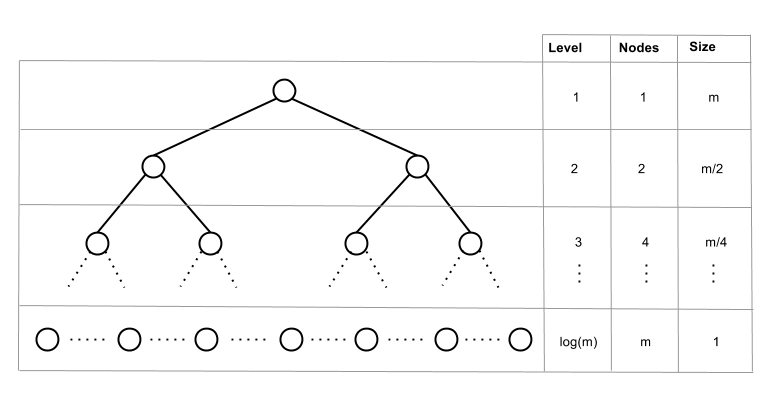
\includegraphics[width=100mm]{../gfx/Tree_level_development.png}

\caption{Development of subtasks as the kd-tree generation progresses. It shows, at each tree level, how many nodes there is to parallelize and how big each node balancing is. }
\label{fig:tree_level_development}
\end{figure}


% TODO: change heading
\subsubsection{Parallelization on CUDA} % (fold)
\label{ssub:divide_work_on_cuda}


CUDA have a special architecture that should be taken into account when parallelizing an algorithm. To efficiently use CUDA the program has to keep thousands of threads occupied, otherwise the benefit of CUDA disappears. The CUDA programming model is build up by a grid if independent block, i.e.\ execution can not be synchronized across blocks. Execution can only be synchronized between the 1 to 1024 theoretical threads launched inside a block~\cite{cuda_programming_guide}. Thread synchronization is important when multiple threads cooperate on one task, because at some point information has to be exchanged.


Our parallelization strategy stats that we have to balance one tree level after another, since they are dependent. This implies that the threads need to communicate between each tree level. One CUDA kernel should therefore balance a complete tree level. The other alternative would be to build the hole tree in one block, which would restrict our kernel to only one SM\@.

The next step is how to split the tree level balance between the CUDA resources. As we observed in Section~\ref{ssub:parallelization_strategy}, the number of node in a tree level increases with the power of two as we go down the tree. The size of each balance process also decreased with a factor of two. Fig~\ref{fig:tree_level_development} shows that our kernel, the tree balance, changes throughout the build process. First only one node needs to be balanced, e.i only one parallel operation. At the end there are $m$ different nodes to work on. The problem size also changes, at the top it is $m$ per node and  goes towards $1$ as the tree level increases.

This varying problem sizes and subtasks, makes it hard to create a good work distribution between the CUDA resources. At the top part of the tree it is optimal to use many blocks to balance a node, but at the end it is desirable to balance many nodes inside every block. We choose a middle ground, to balance one node in one block. This means that there should be an overall good performance with a pick at the middle three levels.


% subsection divide_work_on_cuda (end)

% TODO: Header must be improved
\subsection{Parallelization of the subtree balance} % (fold)
\label{ssub:selecting_a_algorithm}


Now that the overall parallelization strategy is created, we can start investigate the main and time consuming operation, balancing a tree level. We have already determent that the parallelization should be done in one block, which means that one operation is done per SM\@. In other words, the task can potentially be parallelized between 1024 theoretical threads. Lets start investigating different approaches.

The main operation is to find a median. As we have seen in Section~\ref{sub:application_of_kd_trees_to_the_knn_problem}, many algorithms for finding median exist. Since we now want to implement the algorithm with CUDA, the environment has changed, and quick select may not be the best alternative anymore. The first problem with quick select is that it is recursive, which makes it hard to parallelize on CUDA\@. Therefor it may be profitable to look at other, more parallelization friendly, algorithms.


First a reuse of the bitonic sort was investigated. Given a sorted list one can find the median directly, by simply looking at the midmost element of the array. The partitioning is also done in the process. Unfortunately this strategy proved unsuccessful, as re-purposing the bitonic algorithm for such an task proved difficult. The reason for this is that a pure bitonic sorting network only manage to sort lists with a length of power of two. The normal solution is to create a longer list then needed, which destroys many of the advantages with our binary tree representation. There are also other solutions to the problem, for example one by K.E. Batcher~\cite{Batcher:1968}, but these solutions introduces a lot of divergence that destroys performance on the GPU\@. We also have the inherent downside of sorting a list in order to find the median, since \BigO{m} algorithms for finding the median exist, compared to the \BigO{m log(m)} time required by sorting.


The existing linear algorithms for finding the median is mostly based on a more generic problem, namely selection or k'th order statistic algorithms \citep[Chapter 9]{Cormen:2001}. Our serial choice, Quick select, is one of these. It is possible to implement a iterative version, so that the bad properties from the recursive version are eliminated. This option was ignored, because literature states that there are other better suited algorithms, like Alabi \citep{Alabi:2012}. Alabi goes through the radix select and bucket select algorithm in detail. The big difference between them is the constant time penalty. The radix sort have a more exact time complexity of \BigO{bm}, where b is the number of bits in each number. While the penalty for bucket select is \BigO{am}, where $a$ stands for the degree of agglomeration in the values. In other words, the algorithm is week when the points are clusters together. His results shows that bucket select normally is slightly faster, except when $a$ is high. Although bucket select normally have better results, we expect a high degree of agglomeration in our application, so we choose radix select.


\subsubsection{Radix select} % (fold)
\label{ssub:radix_select}

% subsection radix_select (end)

The radix select is based on a bitwise partitioning, much like radix sort~\cite[Chapter 8.3]{Cormen:2001}. In each step, elements are partitioned in two subgroups based on the current bit. Then the subgroup that contains the median is determined, and the search continue in that subgroup until the median is found.

\begin{figure}[ht!]
\centering
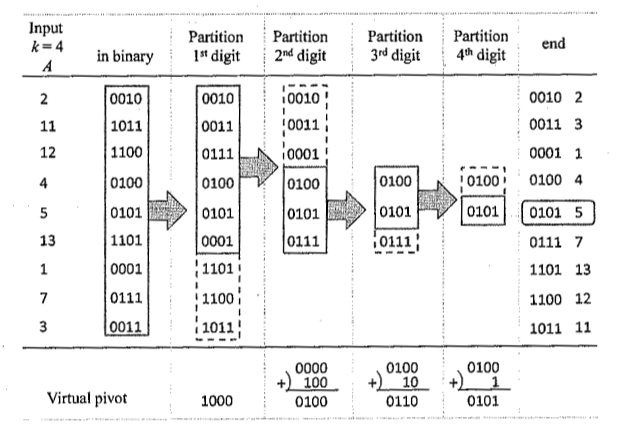
\includegraphics[width=100mm]{../gfx/Radix_select.png}

\caption{An illustration of radix selection\cite{cayman:2012}.}
\label{fig:radix_select}
\end{figure}

When it comes to create a parallelization strategy for radix select it is first advisable to take a look at a highly optimized radix sort like, \citep{MerrillG11}. The radix select can easily be reduced from a radix sort, and many concepts can therefore be reused. An other interesting implementation is the radix select from \citep{Alabi:2012}. They both uses a intuitive parallelization strategy by splitting each radix partition into parallel operations. The way our and Alabi's solution differs from Merrill is firstly that we start on the most significant digit, since a least significant digit approach will not reduce the k'th order statistic problem in each step. Secondly we only iterate on the digit which contains the median, which let us reduce the problem in each iteration.

Our radix select is a slightly modified version in three ways. We want to solve the node task, which forces us to also partition the list around the median. The algorithm also need to work in a in place fashion. The last modification, is that our parallel operation must to several radix selections at once, at different parts of the main tree array.


\subsubsection{Our implementation} % (fold)
\label{ssub:our_implementation}


 % TODO: ta med bigO calculasjon på hele algorithmen.? eller skal vi ha det  i result delen?

Our implementation is based around three different operations that call each other. First we launch a CUDA kernel for each tree level, then the kernel partition the subtrees into different blocks, and the subtree gets balanced. The two first operations is just a partitioning and dividing of resources, as we have talked about in the previous sections. The complete implementation can be found in Appendix~\ref{sec:paralell_k_d_tree_build}. The interesting and time consuming operation is to balance a subtree and is what to be addressed in this section.


Lets take a deeper look into the Algorithm~\ref{alg:parallel_balance_subtree}, that describes the main implementation details in the balance subtree operation. The algorithm only runs inside a block, which means we have a uniform environment with synchronizable threads. The algorithm is based around a repeat-until loop, which basically do all the work. The loop keeps track of a partition array. This array is then sliced in to, by giving each thread a portion of the array, each thread then counts how many zeros it finds in the current bit position. The cut, as the arrows in Figure~\ref{fig:radix_select} shows, is calculated by doing a reduce sum operation \citep{parallel_reduction_in_cuda}. This is repeated until the partition contains the median, which is when every bit is used or when the partition size is one. After the loop, the array is transformed. Such that the median is in the center, with lesser elements on the left and bigger on the right.

\begin{algorithm}[ht]
\caption{Parallel subtree balance}
\label{alg:parallel_balance_subtree}
\begin{algorithmic}
    \Require{A subtree $S$ of length $m$, and dimension $d$}
    \Ensure{A balanced subtree, $S$}
    \Function{Balance-Subtree}{$T$, $d$}
        \State Let $l$ and $u$ be the upper and lower bond of current partition.
        \State Let $P$ be all nodes in $S$
        \Repeat
            \ForAll {$\{p \in P \mid p > l \land p<u\}$}
                \State $Z(t) \gets $  \text{Occurrences of zeros in current bit, $b$, found by thread, $t$.}
            \EndFor
            \State $c \gets \Call{Sum-Reduce}{Z}$ \Comment{$c$ is the cut of the current partition $P$.}
            \If{$u-c >= m/2$}
                \State$ u \gets u-c$
            \Else
                \State$l \gets u-c$
            \EndIf
            \State $b \gets b+1$ \Comment{Move to the next bit}
            \State \Call{Synchronize-Threads}{\ }
        \Until{$u-l<1 \lor b > \Call{Radix}{p \in P} $}
        \State \Call{Partition}{$S, P$}
    \EndFunction
\end{algorithmic}
\end{algorithm}


Some key elements, in regard of CUDA\@, is wort highlighting. In CUDA thread instruction run sequentially in warps of 32. Control flow divergence within a warp can therefore significantly destroy the instruction throughput. This is because the different execution paths must be serialized, as all the thread in a warp share the same program counter\cite{cuda_c_best_practices_guide}. The total number of instruction, in a warp, will therefore increase. Any control flow operator, like for example if, switch and while, should be used with care. In our code, as is necessary in almost all programs, many of these operators are use. It does not directly state that the code is slow, it all depends on how one structure the control operators. In our code one sees that all threads do the same thing in every iteration, the thread branching is small. The loop is also almost done equal times by all thread, one time for each bit used to represent the points. The one $if$ statement in the iteration, can be reduced to only contain one statement, which make the divergent thread branch small. The code is therefore good in regard of divergence.

An other aspect of CUDA is the memory hierarchy. One should always use the fastest and most subtable memory. In our case, this include the shared memory, which is a fast memory shared between all threads in a block. The downside is the memory size, it may not be enough space to store our subtree. Although we may not be able to store the hole subtree, there are some date we can put in the shared memory. The zero counter array, shown as $Z(t)$ in Algorithm~\ref{alg:parallel_balance_subtree}, is a perfect candidate. Every thread only use one integer and it is shared between all threads throughout the execution. It will therefore cause a big impoverishment.

The  complete algorithm can be found in Appendix~\ref{sec:multiple_radix_select}.



% subsection our_implementation (end)

%%%%%%%%%%%%%%%%%%%%%%%%%%%%%%%%%%%%%%%%%%



\subsection{Further improvements} % (fold)
\label{ssub:further_development}


Now that a parallel implementation of the k-d three is ready, lets take a step back and look at our RQ~\ref{rq:parallel_build}. The possibility of parallelizing the build algorithm is achieved, but it is possible to increase the speedup. Are there weaknesses in the code that needs improvement? The best way to investigate these questions is to set up a test, analyze the results.

\begin{figure}[ht!]
\centering
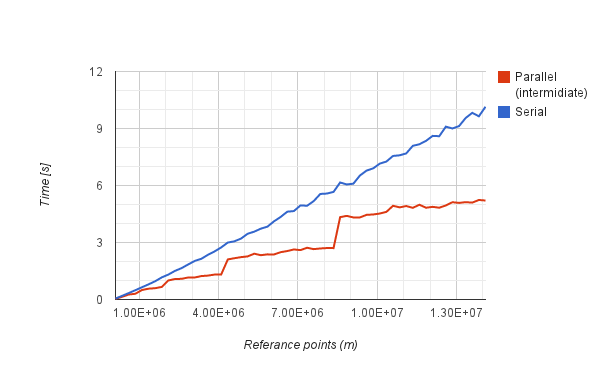
\includegraphics[width=100mm]{../gfx/the_jumps.png}

\caption{Timing results from a intermediate version of the parallel k-d tree build algorithm.}
\label{fig:gpuv1_vs_cpu}
\end{figure}


With the test setup as described in Section~\ref{sec:test_environment}, the current version of the algorithm gave results as shown in Figure~\ref{fig:gpuv1_vs_cpu}. The most interesting observation are the big jumps in the graph. If one look closely these jumps happens every time the problem size exceeds a power of two, as for example when the size passes $8388608$ the timing increases from $2703 ms$ to $4335 ms$. To inveterate this characteristic even further, Table~\ref{tbl:nvprc_balance_branch}, can be used. It shows how long time each tree level takes, and how the different tree level operations varies throughout the build process.

\begin{table}[ht]
\centering
    \begin{tabular}{|l|l|l|l|}
        \hline
        \textbf{Tree level} & \textbf{Time [ms]} & \textbf{Subtrees} & \textbf{Size}\\ \hline
        1          & 52       & 1                  & 1000000      \\ \hline
        2          & 26       & 2                  & 500000       \\ \hline
        3          & 13       & 4                  & 250000       \\ \hline
        4          & 8        & 8                  & 125000       \\ \hline
        5          & 7        & 16                 & 62500        \\ \hline
        6          & 6        & 32                 & 31250        \\ \hline
        7          & 6        & 64                 & 15625        \\ \hline
        8          & 6        & 128                & 7812         \\ \hline
        9          & 7        & 256                & 3906         \\ \hline
        10         & 7        & 512                & 1953         \\ \hline
        11         & 8        & 1024               & 976          \\ \hline
        12         & 10       & 2048               & 488          \\ \hline
        13         & 16       & 4096               & 244          \\ \hline
        14         & 26       & 8192               & 122          \\ \hline
        15         & 52       & 16384              & 61           \\ \hline
        16         & 105      & 32768              & 30           \\ \hline
        17         & 202      & 65536              & 15           \\ \hline
        18         & 389      & 131072             & 7            \\ \hline
        19         & 768      & 262144             & 3            \\ \hline
    \end{tabular}
    \caption{Development of a k-d tree build with a million points, showing how the different tree level operations varies throughout the build process.}
    \label{tbl:nvprc_balance_branch}
\end{table}

The table reviles some weaknesses of our algorithm, that is based around how the CUDA resources was divided in Section~\ref{ssub:divide_work_on_cuda}. It performs badly when the problem size or the number of subtrees is relatively huge. The potential for parallelizing the workload for the first and last iterations is not being fully utilized. This is due to the implementation forcing one version of the radix select algorithm to work on all problem types. This is not optimal for dividing CUDA resources, and as a result, we get high penalties when the problem reaches unsuitable values.

This can also explain the big jumps. The observation correlates perfectly with the tree hight, since the hight of a binary tree is the binary logarithm of the tree size. It implies that the jumps happens when the tree hight is increased and a new tree level needs to be balanced. This increase hits our implementation at it's weakest.

Tuning the algorithm to alternate between different algorithms to balance a subtree, eliminates this problem. This removes the penalty for calculating the median at unsuitable problem sizes. As the are two unstable situation, two different improvements are needed.

Firstly the tree levels with few subtrees and many elements is addressed. Our current implementation only used one block per subtree, which means we are only able to use one SM to balance the subtree. This can be solved by creating a new version that uses all blocks at a time. Big subtrees should then be processed fast, but we get a drawback. Since all blocks are used to balance one subtree, only one subtree can be balanced at a time.

The deep and specific implementation detail will not be fully discussed, but can be found in Appendix~\ref{sec:radix_select}. The overall strategy is pretty similar to the other radix select implementation, except that the thread synchronization has to be done between kernel launches. In an implementation point of view this means that half the code must be implemented on the CPU and the other half on the GPU\@.

The other improvement is to address the other weakness, namely the instance where there are many small subtrees. If one look at the current test results,  Table~\ref{tbl:nvprc_balance_branch}, the problems in hand is in the bottom section. For instance, at level $18$ there are $131072$ different subtask with only an average size of $7$. The previous implementation divided all these subtask between a small number of SM, typically $8-32$ on current NVIDIA GPUs\@. Then the algorithm uses to many cores to balance a subtree of only $7$ elements, which is an extreme bad way of dividing resources.

The solution is to let one thread handle a subtree. That way the CUDA resources is divided in a more suitable manner. This way each thread is responsible for it's own subtree and the need to communicate between other threads is no longer needed. The reasons for not using our serial implementation, Algorithm~\ref{alg:seriel_tree_build}, is therefore gone and we can therefore use it in our parallelization. Only some minor details, subtask dividing and data splitting is needed, as the implementation in Appendix~\ref{sec:parallel_quick_select} shows.



% subsection further_development (end)


% It is hard to use all the parallel power of cuda in this algorithm. The reason is that the problem is divided in three different types; partition one huge list, partition some middle sized list and partition many small lists. This is the reason why we have chosen to use three different implementation of k'th order statistic. The constant time penalties of the two algorithms we have chosen give us a clear indication the radix select is best on large lists while quick select is best on small lists.

% Results:
% \begin{figure}[ht!]
% \centering
% 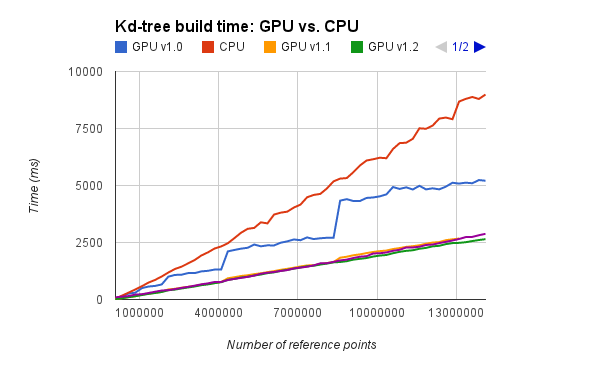
\includegraphics[width=120mm]{../gfx/gpu-vs-cpu-build-time.png}

% \caption{GPU vs CPU build time.}
% \label{fig:sublime_ide}
% \end{figure}

%

% % subsection selecting_a_algorithm (end)
% Memory usage:

% To analyses the space complexity of the k-d tree build and search algorithm, we have made an theoretical calculation of both algorithms GPU memory consumption, and tested it against results from a GeForce 560ti and a Nvidia grid K520 (amazon web service delved).

% It is important to note that the only hard memory limitation is related to building the tree, as a search for N query-points can be performed in several operations. If you e.g. run into memory limitations when searching for pow(10, 8) query-points, you can simply perform two searches on pow(5, 8) query-points to get around the limitation. Loading the pre-built k-d tree on the GPU for searching, and performing one query for a low value of k, will always consume less memory than building the actual k-d tree.

% **Kd-tree-build**

% The memory consumption for the k-d tree build is only depended on the number of points (n) and the theoretical consumption rate grows linearly as \BigO{36n} subset of \BigO{n}.

% \begin{figure}[ht!]
% \centering
% 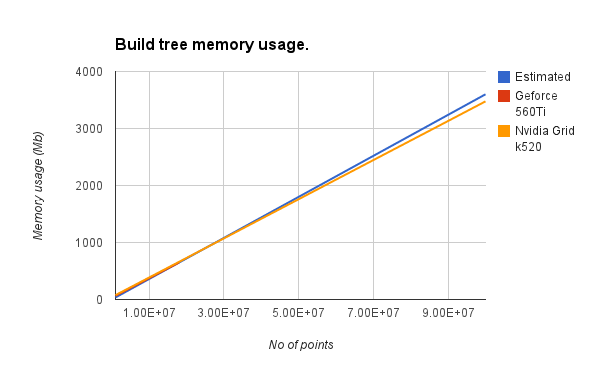
\includegraphics[width=120mm]{../gfx/memory-usage-build.png}

% \caption{Memory usage of k-d tree-build.}
% \label{fig:memory_usage_build}
% \end{figure}

% We see that the estimation fit the real consumption almost perfectly, and with this memory model, we can easily estimate the GPU memory requirements for different problem sizes.

% Given that a customer wants to perform a knn-search on a point cloud of 100 million, he or she would need a GPU with at least 3.6 Gb of spare memory. Under we have tabulated what maximum problem sizes you would expect to be able to run on a selection of Nvidia graphics cards:

% \begin{center}
%     \begin{tabular}{ | l | l | p{5cm} |}
%     \hline
%     Nvidia GPU & Available memory & Maximum problem size \\ \hline
%     GTX TITAN & 6144 MB & 1.79E+08 \\ \hline
%     GTX 780 & 3072 MB & 8.95E+07 \\ \hline
%     GTX 770 & 2048 MB & 5.97E+07 \\ \hline
%     Quadro K6000 & 12288 MB & 3.58E+08 \\ \hline
%     Quadro K5000 & 4096 MB & 1.19E+08 \\ \hline
%     Quadro K4000 & 3072 MB & 8.95E+07 \\ \hline
%     Tesla K40 & 12288 MB & 3.58E+08 \\ \hline
%     Tesla K20 & 5120 MB & 1.49E+08 \\ \hline
%     \end{tabular}
% \end{center}

% These numbers should be read as rough estimates, as each card is expected to have internal processes requiring an unspecified constant amount of the available memory, therefor lovering the maximum problem size possible to run on these cards in practice. It is also worth to mention that when buying a GPU for GPGPU tasks, other performance characteristics is equally, or more, important.

% **Kd-search**

% The kd-search is used to query every point against each other. It has a theoretical memory consumption rate at \BigO({40+4k}n) subset of \BigO{kn}. The consumption is therefore depended on the number of points (n) and the number of neighbors (k).

% \begin{figure}[ht!]
% \centering
% 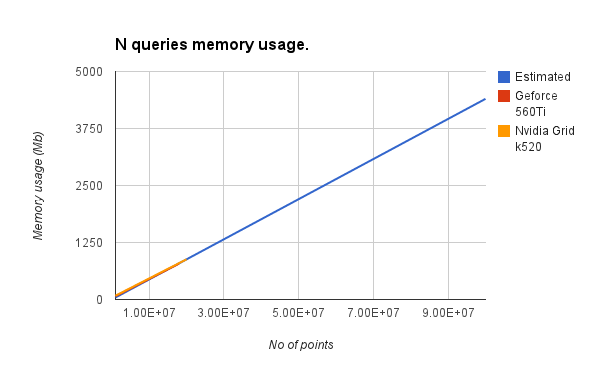
\includegraphics[width=120mm]{../gfx/memory-usage-kd-search.png}

% \caption{Memory usage of kd-search.}
% \label{fig:memory-usage-kd-search}
% \end{figure}

% Also in this case our estimation fit the real consumption with a high degree of accuracy.

% Further work:
% \begin{itemize}
%     \item Look at memory optimization.
%     \item Improve utiliti methods like: accumulateindex, minReduce.
%     \item Forloop Unrolling.
% \end{itemize}
